\documentclass[12pt,a4paper]{article} 
\usepackage{a4wide}
\usepackage[utf8]{inputenc}
\usepackage{amsmath}
\usepackage{amsfonts}
\usepackage{amssymb}
\usepackage{graphicx}
\usepackage{float}
\usepackage[ngerman]{babel} 
\usepackage{pdflscape}
\usepackage{caption, booktabs}
\parindent0pt


\title{Teilentwurf von  LISE E-Learning System}

\author{Matthias Englert, Fabian Schilha, Andreas Rottach}
\date{Wintersemester 2014/2015}

\begin{document}
\maketitle
\newpage
\tableofcontents
\newpage

\section{Datenbankentwurf}

\subsection{Datebankdiagramm}
\begin{figure}[H]
	\centering
	\paragraph{Aufbau der Relationalen Datenbank}	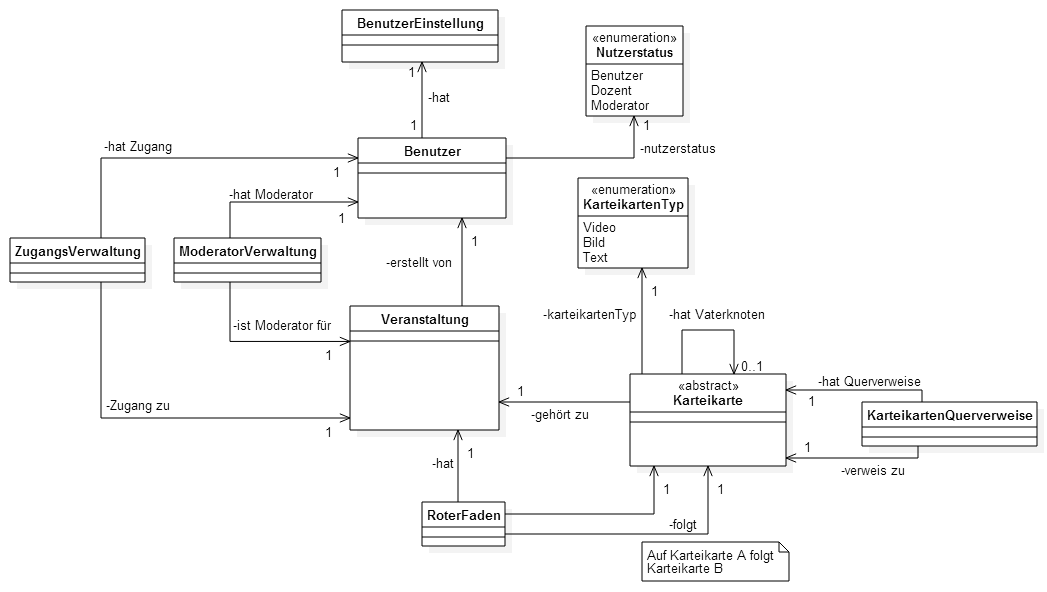
\includegraphics[width=\textwidth]{Bilder/Datenbank/Datenbankentwurf.png}
	\caption{Datenbankdiagramm}
	\label{Datenbankdiagramm}
\end{figure}

\subsection{Beschreibung der Tabellen}

\begin{tabular}{|lp{12cm}|}
	\hline
	TABELLE			&  Benutzer\\ 
	BESCHREIBUNG	&  Speichert alle Informationen, die zu einem Benutzer gehören.\\ 
	VERWALTET		& Benutzerdaten\\ 
	SCHLÜSSEL		&  ID : Integer\\ 
	\hline
	&  \\ 
	FELD		    &  Vorname : String\\  
	&  \\ 
	FELD		    &  Nachname : String\\  
	&  \\ 
	FELD		    &  Martrikelnummer : Integer\\  
	&  \\
	FELD		    &  eMail : String\\ 
	BESCHREIBUNG	&  Veranstaltungsbeschreibung\\
	&  \\
	FELD		    &  Studiengang : Enum\\ 
	BESCHREIBUNG	&  Fremdschlüssel, Benutzer ist bestimmtem Studiengang zugeordnet. Dozenten sind hier keinem Studiengang zugeordnet. Referenziert auf Tabelle Studiengang\\ 
	&  \\
	FELD		    &  Kennwport : String\\ 
	BESCHREIBUNG	&  Speichert das verschlüsselte Passwort des Nutzers \\
	&  \\
	FELD		    &  Nutzerstatus : Enum\\ 
	BESCHREIBUNG	&  Speichert ob Benutzer ein Student oder Dozent ist.\\
	&  \\
	FELD		    &  GruppeneinladungenErlauben : Bool\\ 
	BESCHREIBUNG	&  Speichert ob Benutzer zu Gruppen eingeladen werden kann.\\
	&  \\
	FELD		    &  NotifyDiskussionen : Enum\\ 
	BESCHREIBUNG	&  Speichert wie ein Benutzer über Diskussionen informiert wird.\\
	\hline
\end{tabular}\\\\

\begin{tabular}{|lp{12cm}|}
	\hline
	TABELLE			&  Studiengang\\ 
	BESCHREIBUNG	&  alle Studiengänge an der Universität Ulm\\ 
	VERWALTET		&  Benutzer und deren eingetragenen Studiengang\\ 
	SCHLÜSSEL		&  ID : Integer\\ 
	\hline
	&  \\
	FELD		    &  Studiengang : String\\ 
	BESCHREIBUNG	&  Text der den Studiengang beschreibt.\\
	\hline
\end{tabular}\\\\


\section{System-Architektur}

\subsection{Kommunikationsdiagramm}

\begin{figure}[H]
	\centering
	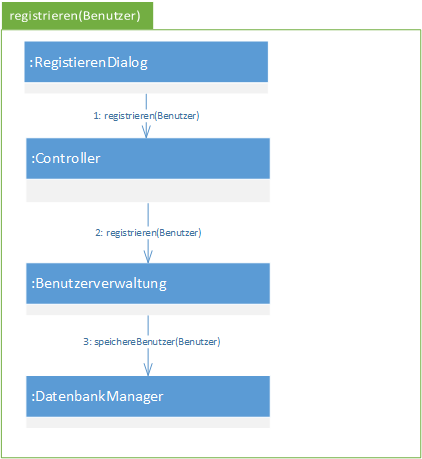
\includegraphics[width=0.7\linewidth]{Bilder/Kommunikationsdiagramme/registrieren}
	\caption{Registrierung}
	\label{Registrierung}
\end{figure}

\begin{figure}[H]
\centering
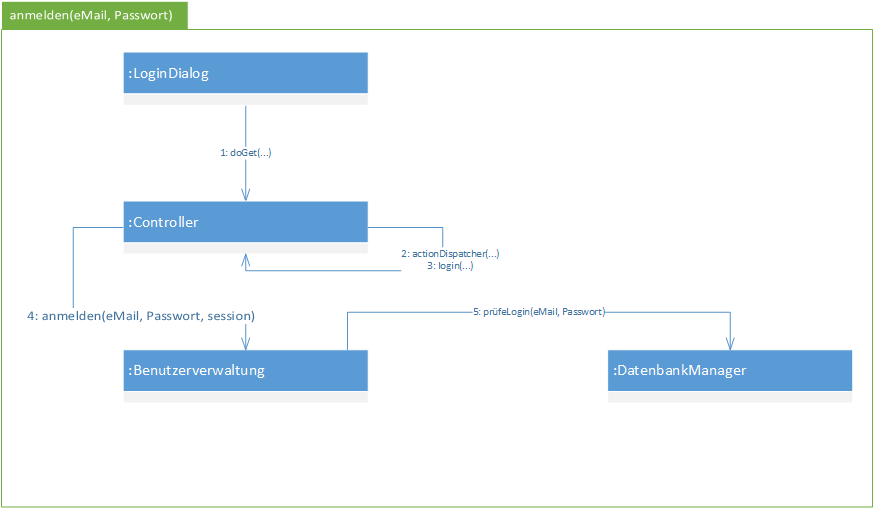
\includegraphics[width=0.7\linewidth]{Bilder/Kommunikationsdiagramme/anmelden}
\caption{Am System anmelden}
\label{Am System anmelden}
\end{figure}


\begin{figure}[H]
\centering
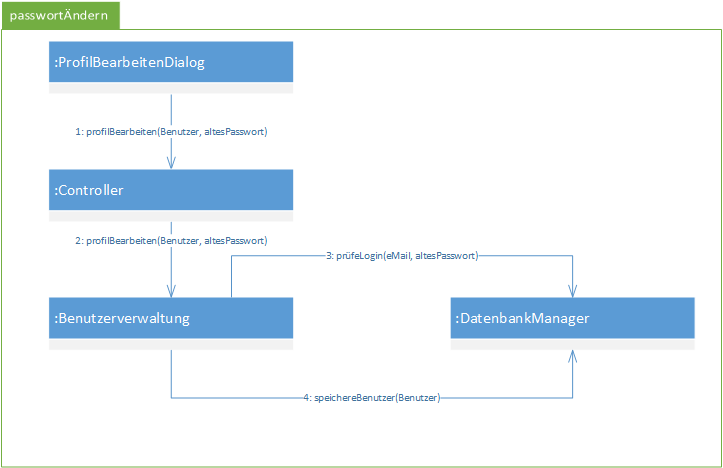
\includegraphics[width=0.7\linewidth]{Bilder/Kommunikationsdiagramme/passwortAendern}
\caption{Passwortänderung}
\label{Passwortaenderung}
\end{figure}




\subsection{Klassendiagramm}

% Klassendiagramm einfügen

\subsection{Methodenbeschreibung}


\paragraph{title}

\begin{tabular}{|lp{12cm}|}
			\hline
			Operation &  \textbf{registrieren(neuerNutzer: Benutzer): Boolean }\\ 
			Beschreibung & Ein Benutzer registriert sich neu im System und gibt alle verlangten Daten an. Die Operation prüft ob die Daten korrekt sind und legt den neuen Benutzer gegebenenfalls an.\\ 
			\hline 
\end{tabular} \\\\


\begin{tabular}{|lp{12cm}|}
	\hline
	Operation &  \textbf{profilAnzeigen() }\\ 
	Beschreibung & Ein Benutzer registriert sich neu im System und gibt alle verlangten Daten an. Die Operation prüft ob die Daten korrekt sind und legt den neuen Benutzer gegebenenfalls an.\\ 
	\hline 
\end{tabular} \\\\



\end{document}
